\documentclass[11pt,twocolumn]{article}
    \usepackage{fontspec} %connects to native fonts
    \usepackage{amsmath}
    \usepackage{mathtools}
    \usepackage{cleveref}
    \usepackage{pgfplots}
    \usepackage{graphicx}
    \usepackage{wrapfig}
    \usepackage{fancyref}
    \usepackage{amssymb}
    \usepackage{subfig}
    \usepackage{float}
    \usepackage[justification=RaggedRight, singlelinecheck=false, font={footnotesize}]{caption}
    \usepackage[portuguese]{babel}
    \usepackage[title,titletoc,toc]{appendix}
    \usepackage{fontspec}
    \begin{document}
    \pagenumbering{arabic}
    \bibliographystyle{plain}
    \title{
        \textnormal{
        \LARGE Universidade de Lisboa - Instituto Superior Técnico\\
        \Large Licenciatura em Engenharia Informática e de Computadores\\
        \Large Inteligência Artificial
    \\}
        \LARGE2º Projeto - Grupo 22
        \vspace{-1ex}
        }
    \author{Gonçalo Marques,
        \texttt{84719}
        \and
        Manuel Sousa,
        \texttt{84740}
    }
    \date{	\vspace{-1ex}
            \vspace{-4ex}
        }
    \maketitle
    
    \section*{P1}
    
    Começámos por elaborar um conjunto de features a aplicar sobre as palavras. De inicio contruímos features básicas que verificassem o numero de vogais e consoantes de uma palavra, o numero de acentos, etc. O primeiro objetivo passava apenas por estudar
    o comportamento do avaliador, e durante este processo, facilmente concluímos que quanto mais único fosse o output da feature em relação à palavra recebida, menor seria o erro.
    
    
    \begin{table}[htbp]
        \centering
        \caption{Analise individual dos erros de cada feature}
        \label{my-label}
        \begin{tabular}{|l|c|c|}
        \hline
        \multicolumn{1}{|c|}{Features Individuais}     & \textbf{Teste 1} & \textbf{Teste 2}                    \\ \hline
        [F1] N Acentos & 0.666   & 0.231 \\ \hline
        [F2] N Vogais Par & 0.264   & 0.231 \\ \hline
        [F3] N Vogais & 0.264   & 0.348 \\ \hline
        [F4] N Consoantes   & 0.264  & 0.231      \\ \hline
        [F5] Palavras Repetidas   & 0.264  & 0.231      \\ \hline
        [F6] Palavra Par   & 0.231  & 0.231      \\ \hline
        [F7] Soma ASCII                             & 0.130            & 0.122                                \\ \hline
        [F8] Hash                             & 0.0              & 0.0                                 \\ \hline
        \end{tabular}
        \end{table}
    \par

    Podemos observar que a função que soma o ASCII dos caracteres
    constituintes da palavra, tem um erro muito reduzido visto que o output dado pela feature será sempre único, menos quando palavras diferentes são constituídas pelos mesmos caracteres. 
    Assim, uma função que der um output único para cada palavra recebida iria dar um erro ainda mais baixo. Criámos uma função que gera um inteiro único para uma palavra (Hash), e desta maneira conseguimos obter uma percentagem de erro de 0\%.
    
    \begin{table}[htbp]
        \centering
        \caption{Analise coletiva dos erros com várias features}
        \label{my-label}
        \begin{tabular}{|l|c|c|}
        \hline
        \multicolumn{1}{|c|}{Features Coletivas}         & \textbf{Teste 1} & \textbf{Teste 2}                    \\ \hline
        [F5] + [F6] & 0.231 & 0.231 \\ \hline
        [F5] + [F6] + [F7]     & 0.077  & 0.077                   \\ \hline
        [F4] + [F5] + [F7] + [F8]   & 0.0              & 0.0                                 \\ \hline
        [F3] + [F4] + [F7]   & 0.064             & 0.064                                 \\ \hline
        [F3] + [F4] + [F7] + [F8]   & 0.0          & 0.0                                 \\ \hline
        \end{tabular}
        \end{table}
    \par  
    Por observação à tabela concluímos que a utilização de várias features produz um erro mais baixo, que usar features individuais. 
    Observamos também que a feature 8 é predominante, visto que a sua presença é suficiente para dar erro de 0\%. De forma a obter os melhores resultados (excluindo a feature 8), fomos ajustando as várias features até obter o melhor resultado possível.

\section*{P2}

Texto.

\section*{P3}

A imagem seguinte ilustra como o agente se movimenta pelo ambiente 1, incluíndo uma representação gráfica do mesmo:

\begin{center}
    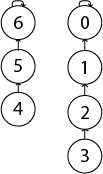
\includegraphics[scale=0.4]{Trajetoria1.png}
\end{center}

\par A imagem seguinte ilustra como o agente se movimenta pelo ambiente 1, incluíndo uma representação gráfica do mesmo:



\begin{center}
    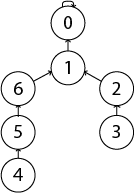
\includegraphics[scale=0.4]{Trajetoria2.png}
\end{center}

A função de recompensa é a seguinte para ambas as trajetórias 

\begin{center}
    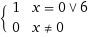
\includegraphics[scale=0.6]{piece1.png}
\end{center}

\end{document}
